
%(BEGIN_QUESTION)
% Copyright 2010, Tony R. Kuphaldt, released under the Creative Commons Attribution License (v 1.0)
% This means you may do almost anything with this work of mine, so long as you give me proper credit

Something is wrong with this valve control circuit.  When the operator presses the ``open'' pushbutton, the valve position indicating lights still show it to be closed (green light on, red light off):

$$\includegraphics[width=15.5cm]{i01564x01.eps}$$

Determine the diagnostic value of each of the following tests.  Assume only one fault in the system, including any single component or any single wire/cable/tube connecting components together.  If a proposed test could provide new information to help you identify the location and/or nature of the one fault, mark ``yes.''  Otherwise, if a proposed test would not reveal anything relevant to identifying the fault (already discernible from the measurements and symptoms given so far), mark ``no.''

% No blank lines allowed between lines of an \halign structure!
% I use comments (%) instead, so that TeX doesn't choke.

$$\vbox{\offinterlineskip
\halign{\strut
\vrule \quad\hfil # \ \hfil & 
\vrule \quad\hfil # \ \hfil & 
\vrule \quad\hfil # \ \hfil \vrule \cr
\noalign{\hrule}
%
% First row
{\bf Diagnostic test} & {\bf Yes} & {\bf No} \cr
%
\noalign{\hrule}
%
% Another row
Measure AC voltage across Fuse F1 &  &  \cr
%
\noalign{\hrule}
%
% Another row
Measure AC voltage across Fuse F3 &  &  \cr
%
\noalign{\hrule}
%
% Another row
Measure AC voltage across solenoid coil with ``Open'' button pressed &  &  \cr
%
\noalign{\hrule}
%
% Another row
Measure AC voltage across solenoid coil with ``Closed'' button pressed &  &  \cr
%
\noalign{\hrule}
%
% Another row
Measure AC voltage between terminals X2 and T with ``Open'' button pressed &  &  \cr
%
\noalign{\hrule}
%
% Another row
Measure AC voltage between terminals L and D with ``Open'' button pressed &  &  \cr
%
\noalign{\hrule}
%
% Another row
Check air supply pressure (look at pressure gauge) &  &  \cr
%
\noalign{\hrule}
} % End of \halign 
}$$ % End of \vbox

\vfil 

\underbar{file i01564}
\eject
%(END_QUESTION)





%(BEGIN_ANSWER)

This is a graded question -- no answers or hints given!

%(END_ANSWER)





%(BEGIN_NOTES)

A good problem-solving strategy to use in cases like this where we must assess the appropriateness of various diagnostic tests is to first determine what might be faulted in this circuit, and what we know to be good.  Only then will we be able to determine whether or not a particular test will provide us with new information about the fault (the criterion for a valid diagnostic test).

For example, the fact that the green light is energized tells us the circuit has power.  This means, among other things, that fuses F1, F2, and F4 are all good.  Therefore, any measurement of AC voltage across F1 is a bad test, because we already know from the green lamp's illumination that fuse F1 must be good and therefore it will all drop (nearly) zero volts.

% No blank lines allowed between lines of an \halign structure!
% I use comments (%) instead, so that TeX doesn't choke.

$$\vbox{\offinterlineskip
\halign{\strut
\vrule \quad\hfil # \ \hfil & 
\vrule \quad\hfil # \ \hfil & 
\vrule \quad\hfil # \ \hfil \vrule \cr
\noalign{\hrule}
%
% First row
{\bf Diagnostic test} & {\bf Yes} & {\bf No} \cr
%
\noalign{\hrule}
%
% Another row
Measure AC voltage across Fuse F1 with ``Closed'' button pressed &  & $\surd$ \cr
%
\noalign{\hrule}
%
% Another row
Measure AC voltage across Fuse F3 with ``Closed'' button pressed & $\surd$ &  \cr
%
\noalign{\hrule}
%
% Another row
Measure AC voltage across solenoid coil with ``Open'' button pressed & $\surd$ &  \cr
%
\noalign{\hrule}
%
% Another row
Measure AC voltage across solenoid coil with ``Closed'' button pressed &  & $\surd$ \cr
%
\noalign{\hrule}
%
% Another row
Measure AC voltage between terminals X2 and T with ``Open'' button pressed &  & $\surd$ \cr
%
\noalign{\hrule}
%
% Another row
Measure AC voltage between terminals L and D with ``Open'' button pressed & $\surd$ &  \cr
%
\noalign{\hrule}
%
% Another row
Check air supply pressure (look at pressure gauge) & $\surd$ &  \cr
%
\noalign{\hrule}
} % End of \halign 
}$$ % End of \vbox

\vskip 20pt \vbox{\hrule \hbox{\strut \vrule{} {\bf Virtual Troubleshooting} \vrule} \hrule}

This question is a good candidate for a ``Virtual Troubleshooting'' exercise.  Presenting the diagram to students, you first imagine in your own mind a particular fault in the system.  Then, you present one or more symptoms of that fault (something noticeable by an operator or other user of the system).  Students then propose various diagnostic tests to perform on this system to identify the nature and location of the fault, as though they were technicians trying to troubleshoot the problem.  Your job is to tell them what the result(s) would be for each of the proposed diagnostic tests, documenting those results where all the students can see.

During and after the exercise, it is good to ask students follow-up questions such as:

\begin{itemize}
\item{} What does the result of the last diagnostic test tell you about the fault?
\item{} Suppose the results of the last diagnostic test were different.  What then would that result tell you about the fault?
\item{} Is the last diagnostic test the best one we could do?
\item{} What would be the ideal order of tests, to diagnose the problem in as few steps as possible?
\end{itemize}


%INDEX% Troubleshooting review: electric circuit diagnostic test usefulness

%(END_NOTES)


